\chapter{UML-Zustandsdiagramme}
\renewcommand{\chaptertitle}{UML-Zustandsdiagramme}

\lehead[]{\sf\hspace*{-2.00cm}\textcolor{white}{\colorbox{lightblue}{\makebox[1.60cm][r]{\thechapter}}}\hspace{0.17cm}\textcolor{lightblue}{\chaptertitle}}
\rohead[]{\textcolor{lightblue}{\chaptertitle}\sf\hspace*{0.17cm}\textcolor{white}{\colorbox{lightblue}{\makebox[1.60cm][l]{\thechapter}}}\hspace{-2.00cm}}
%\chead[]{}
\rehead[]{\textcolor{lightblue}{AvHG, Inf, My}}
\lohead[]{\textcolor{lightblue}{AvHG, Inf, My}}

\lstset{style=myJava}

\section{Notation}

Ein UML-Zustandsdiagramm beschreibt die Zustände eines Objektes. Bei der
Umsetzung des Zustandsdiagramms in ein Programm nummeriert man die einzelnen
Zustände durch und fügt im Code eine Integer-Variable ein, in der die Nummer
des aktuellen Zustands gespeichert wird.


\subsection{Darstellung der Zustände}

\bgroup
\def\arraystretch{1.2}
\begin{tabular}{lp{55mm}p{62mm}}
\textbf{Schema:} &
\vspace{-6mm}
\begin{center}
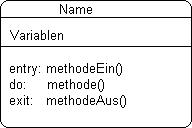
\includegraphics[width=0.3\textwidth]{./inf/SEKII/11_UML_Zustandsdiagramme/schemaZustand.png}
\end{center}
&
Hinter \textbf{entry} werden alle Methoden aufgelistet, die
beim Eintritt in den Zustand ausgeführt werden. 

Hinter \textbf{do} werden alle Methoden aufgelistet, die solange
ausgeführt werden, wie der Zustand andauert. 

Hinter \textbf{exit} werden alle Methoden aufgelistet, die beim
Verlassen des Zustands ausgeführt werden.
\\
\textbf{Beispiele:} &
\vspace{-6mm}
\begin{center}
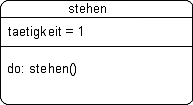
\includegraphics[width=0.3\textwidth]{./inf/SEKII/11_UML_Zustandsdiagramme/beispielStehen.png}
\end{center}
&
\vspace{-6mm}
\begin{center}
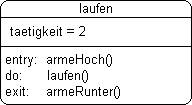
\includegraphics[width=0.3\textwidth]{./inf/SEKII/11_UML_Zustandsdiagramme/beispielLaufen.png}
\end{center}
\\
\textbf{Besondere Zustände:} &
\vspace{-3mm}

\includegraphics[width=0.02\textwidth]{./inf/SEKII/11_UML_Zustandsdiagramme/startzustand.png}
\hspace{2mm} Startzustand
&
\vspace{-3mm}

\includegraphics[width=0.02\textwidth]{./inf/SEKII/11_UML_Zustandsdiagramme/endzustand.png}
\hspace{2mm} Endzustand
\\
\end{tabular}
\egroup


\subsection{Darstellung von Zustandsübergängen}

\bgroup
\def\arraystretch{1.2}
\begin{tabular}{lp{55mm}}
\vspace{4mm}
\textbf{Schema:} &
\vspace{-6mm}
\begin{center}
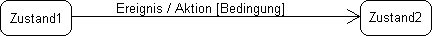
\includegraphics[width=0.6\textwidth]{./inf/SEKII/11_UML_Zustandsdiagramme/schemaZustandsuebergang.png}
\end{center}
\\
\vspace{4mm}
\textbf{Beispiel:} &
\vspace{-8mm}
\begin{center}
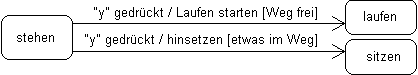
\includegraphics[width=0.6\textwidth]{./inf/SEKII/11_UML_Zustandsdiagramme/beispielZustandsuebergang.png}
\end{center}
\\
\end{tabular}
\egroup


\subsubsection{Beschriftung der Zustandsübergänge}

\bgroup
\def\arraystretch{1.2}
\begin{tabular}{|l|p{130mm}|}
\hline
\textbf{Ereignis} &
Das System wird von außen angestoßen seinen Zustand zu ändern
(in der Regel durch den Benutzer).

Beispiele: Tastendruck, Klick auf einen Button, Signal von der Systemuhr
\\ \hline
\textbf{/Aktion} & 
Tätigkeit, die das System während des Zustandsübergangs
ausführt (z.B. Aufruf einer Methode).
\\ \hline
\textbf{[Bedingung]} &
Das System entscheidet aufgrund von eigenen Informationen
(z.B.\ Variablenwerten), in welchen Zustand es übergeht.
Eine Bedingung ist nur dann sinnvoll, wenn verschiedene Zustände zur Auswahl stehen.
\\ \hline
\end{tabular}
\egroup


\subsection{Zustand oder Zustandsübergang?}

Zustandsübergänge sind extrem kurze Momente. Eine Tätigkeit, die eine längere
Zeitspanne umfasst, muss als Zustand modelliert werden.


\section{Beispiele}

\subsection{Zustandsdiagramme für das Strichmännchen}

Im Kurs-Repository findest du die Dateien \myFile{Maennchen.java} und
\myFile{Main.java}. Kopiere die beiden Dateien in dein eigenes Java-Projekt und
starte das Programm. Du kannst das Männchen mit den Tasten '\lstinline|x| und
'\lstinline|y|' steuern.

\begin{center}
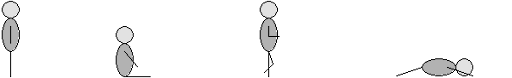
\includegraphics[width=0.8\textwidth]{./inf/SEKII/11_UML_Zustandsdiagramme/maennchen.png}
\end{center}

Das Verhalten des Männchens lässt sich in einem Zustandsdiagramm abbilden.

\begin{compactenum}[a)]
\item Einfaches Zustandsdiagramm

\begin{center}
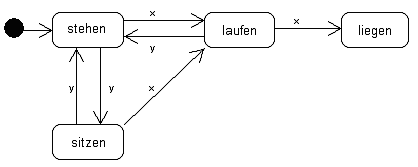
\includegraphics[width=0.5\textwidth]{./inf/SEKII/11_UML_Zustandsdiagramme/zustandsdiagrammMaennchenEinfach.png}
\end{center}

\item Zustandsdiagramm mit Details für die Programmierung

\begin{center}
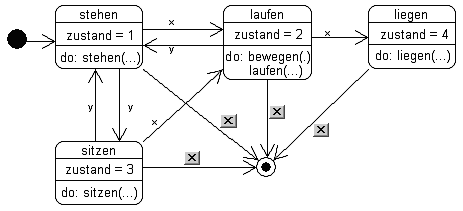
\includegraphics[width=0.6\textwidth]{./inf/SEKII/11_UML_Zustandsdiagramme/zustandsdiagrammMaennchenDetailliert.png}
\end{center}

\end{compactenum}

\pagebreak


\subsection{Komplexes Beispiel}

Zustände eines Objekts der Klasse „Lehrer“:

\begin{center}
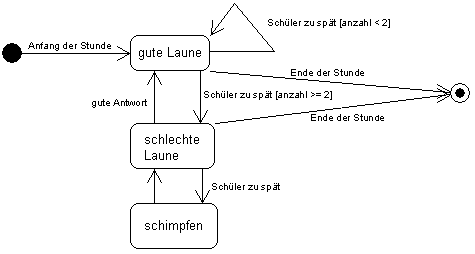
\includegraphics[width=0.6\textwidth]{./inf/SEKII/11_UML_Zustandsdiagramme/zustandsdiagrammLehrer.png}
\end{center}

